% !BIB TS-program = biber

\RequirePackage[l2tabu,orthodox]{nag}

% TODO: decide if one-sided/two-sided
%\documentclass[headsepline,footsepline,footinclude=false,fontsize=11pt,paper=a4,listof=totoc,bibliography=totoc,BCOR=12mm,DIV=12]{scrbook} % two-sided
\documentclass[headsepline,footsepline,footinclude=false,oneside,fontsize=11pt,paper=a4,listof=totoc,bibliography=totoc]{scrbook} % one-sided

% TODO: change citation style in settings
\input{settings}

% TODO: change thesis information
\newcommand*{\getUniversity}{Technische Universität München}
\newcommand*{\getFaculty}{Informatics}
\newcommand*{\getDegree}{Informatics}
\newcommand*{\getSchool}{Computation, Information and Technology}
\newcommand*{\getTitle}{Extension of Prometheus for Scalable and Resilient Black Box Monitoring}
\newcommand*{\getTitleGer}{Erweiterung von Prometheus für skalierbares und belastbares Black-Box-Monitoring}
\newcommand*{\getAuthor}{Jih-Wei Liang}
\newcommand*{\getDoctype}{Master's Thesis}
\newcommand*{\getSupervisor}{Michael Gerndt; Prof. Dr.-Ing.}
\newcommand*{\getAdvisor}{Samuel Torre Vinuesa}
\newcommand*{\getSubmissionDate}{15.03.2024}
\newcommand*{\getSubmissionLocation}{Munich}

\begin{document}

% Set page numbering to avoid "destination with the same identifier has been already used" warning for cover page.
% (see https://en.wikibooks.org/wiki/LaTeX/Hyperlinks#Problems_with_Links_and_Pages).
\pagenumbering{alph}
\input{pages/cover}

\frontmatter{}

\input{pages/title}
\input{pages/disclaimer}
\addcontentsline{toc}{chapter}{Acknowledgments}
\thispagestyle{empty}

\vspace*{20mm}

\begin{center}
    {\usekomafont{sectioning}\usekomafont{section} Acknowledgments}
\end{center}

\vspace{10mm}

%TODO: Acknowledgments

I am profoundly grateful to my advisor, Samuel Torre Vinuesa, whose steadfast guidance and insightful criticism have been instrumental in my journey through this research. His deep knowledge and clear articulation of the subject matter have significantly enhanced my understanding and appreciation of the field. Samuel's support in defining the research topic, structuring the thesis, and navigating the challenges encountered during my research journey has been invaluable. 

Additionally, I extend my heartfelt thanks to my supervisor, Prof. Dr.-Ing. Michael Gerndt, for offering me the chance to conduct my research within the chair of Computer Architecture and Parallel Systems at the Department of Informatics, Technical University of Munich. This opportunity has been pivotal in my academic and professional growth. 

My colleagues at Amadeus Data Processing GmbH deserve special mention for their unwavering support throughout my research. Jerome Mazeries and Gais Ameer's assistance with technical issues and their constructive feedback have been crucial in the completion of my work. I am deeply appreciative of the supportive and collaborative environment they provided. 

Last but certainly not least, I owe a tremendous debt of gratitude to my family. Their moral support and belief in my abilities have been my stronghold. It is their encouragement that fortified my resolve and enabled me to bring this thesis to fruition. 

\cleardoublepage{}

\chapter{\abstractname}

%TODO: Abstract

With IT infrastructures' increasing complexity and scale, Amadeus's traditional monitoring solutions often fail to provide the necessary observability and operational efficiency. To address this gap, a scalable, reliable, and cloud-ready active monitoring platform becomes a need. The research investigates and compares two potential active monitoring solutions: a self-developed system employing operators, schedulers, and probers and a comprehensive solution using the Prometheus Operator, Prometheus Agent, and Blackbox Exporter for advanced cloud integration. The study concludes that with its automated configuration and management capabilities, the Prometheus Operator offers the most alignment with Amadeus's requirements for scalability, reliability, and cloud readiness. It ensures compatibility with custom protocols and optimizes resource usage, notably improving operational efficiency and reducing memory overhead compared to original monitoring methods. The architecture integrates seamlessly with Kubernetes and OpenShift, facilitating efficient deployment and management of monitoring components. A detailed evaluation of active monitoring solutions within a complex IT ecosystem was provided to contribute to the broad monitoring community, highlighting the Prometheus Operator's role in enhancing observability and operational efficacy. Future research will focus on automating Blackbox Exporter configurations, developing interfaces for custom probers, integrating eBPF for precise monitoring, and exploring advanced machine learning and tools tailored for microservices, aiming to enhance the efficiency, flexibility, and observability of monitoring solutions in complex IT environments. 
\microtypesetup{protrusion=false}
\tableofcontents{}
\microtypesetup{protrusion=true}

\mainmatter{}

% \input{chapters/00_example.tex}
% TODO: add more chapters here
% !TeX root = ../main.tex
% Add the above to each chapter to make compiling the PDF easier in some editors.

\chapter{Introduction}\label{chapter:introduction}

System monitoring is essential in the modern \ac{IT} industry. It offers observability to both users and developers, enabling rapid detection and notification of issues. For Amadeus's extensive network of interlinked applications, observability is vital to swiftly identifying, diagnosing, and resolving problems, ensuring our customers receive the highest quality service. 

The Amadeus Observability Platform accommodates a variety of monitoring data, including metrics, logs, structured logs, and events. It is built on the Prometheus ecosystem and integrates with Splunk. Additionally, Amadeus actively contributes to the Prometheus ecosystem. A prime example is Perses, a new CNCF project developed and maintained by Amadeus that aims at observability data visualization. 

Recently, demands for probing on kinds of applications in \ac{ACS} by customized requests, such as those of \ac{HTTP}/\ac{HTTPS}, \ac{DNS}, \ac{ICMP}, \ac{SNMP}, etc, have increased, which stemmed from the increasing focus on observability. This kind of monitoring actively sends simulated requests and observes the response without internal knowledge, which could benefit observability with low cost and fast reaction. As part of the overall strategy for rock-solid operations, Amadeus needs this kind of monitoring on scale. 

As mentioned above, the tendency brings about the demand for introducing Active Monitoring or Black Box Monitoring to Amadeus. By definition, Active Monitoring features the simulation of requests and observation of responses, covering the scope of Black Box Monitoring. However, the two monitoring methods have slight differences in concepts. Active monitoring emphasizes proactively watching the reactions to simulated behaviors~\parencite{splunkActiveVsPassive2023}. On the other side, Black Box Monitoring focuses on ignoring the internal mechanism, only caring about the input and output of the application~\parencite{beyerSiteReliabilityEngineering2016}. In conclusion, although the two monitoring methods have different names and concepts, they still feature similar behaviors and fit the latest monitoring requirements in Amadeus. 

Following alignment meetings with Platform Product Management and Tech Senior Leaders, a consensus was reached regarding the requirements for the final solution in active monitoring. The solution must be highly scalable, reliable, and cloud-ready to meet the needs of a modern \ac{IT} environment. It should support multiple protocols such as \ac{HTTP}, \ac{SOAP}, \ac{REST}, \ac{EDIFACT}, etc. Additionally, the system must be modular to facilitate the easy addition of new protocols.

Additionally, other essential features concerning the Operating Model should be considered. For example, the active monitoring platform must be self-service and fully support “as-code” configurations such as GitOps. Also, it should support deploying probers and selecting their origin and target with an easy interface. Lastly, seamless integration with the Amadeus Observability Platform, including the Event Management stack, is crucial to ensure a cohesive and efficient monitoring ecosystem.

Nowadays, there are renowned tools to implement system monitoring, such as Prometheus, Datadog, Nagios, and so on. These tools aim to collect various metrics from targets for monitoring computational resources. Generally, they provide an agent to scrape desired data and then wait for the server's request or actively push these data to the responsible server. Most of them feature great professions in monitoring, offering enterprise-level services in reaction to kinds of requirements~\parencite{nevesDetailedBlackboxMonitoring2021}.

This project considers two solutions to align with the Amadeus Observability Platform. The first is a customized application with scheduled probings, probing targets, and a centralized user interface. The third solution involves leveraging the Prometheus Operator, the Prometheus Agent, and the Blackbox Exporter to construct an integrated, compatible active monitoring platform. 

The first solution comprises three main components: the Operator, the Scheduler, and the Prober. The Operator is responsible for handling the \ac{CRD} that defines the service and related information for monitoring. The Scheduler is tasked with scheduling monitoring requests based on the \ac{CRD} and collecting data from the Probers. Lastly, the Prober is a custom worker designed for various monitoring purposes. It sends target requests and then returns the data required to the Scheduler. The significant advantage of this method is full customization; however, the disadvantages are the heavy maintenance load and the inconsistency with the open-source framework. 

The second solution mirrors the first with substitutions: the operator for the Prometheus Operator, the scheduler for the Prometheus Agent, and general probers for the Blackbox Exporter, except for certain custom probers designed for specialized protocols by Amadeus. Similar to the first solution's operator, the Operator Pattern facilitates the automation of configuration and management within container orchestration platforms like Kubernetes and OpenShift~\parencite{kubernetesOperatorPattern}. Therefore, the Prometheus Operator helps users deploy and manage the components in the ecosystem, which are needed for active monitoring, achieving sharding and auto scalability without additional effort~\parencite{prometheusoperatorIntroduction2020}. On the other hand, users must understand and utilize official \ac{CRD}s to conduct settings, which brings some learning curve to the promoting. 

In selecting the final solution, the second option involving the Prometheus Operator stands out as the preferred choice for several reasons. Firstly, the Prometheus Operator can be seen as an enhanced and official version of the first solution, offering improved compatibility. Additionally, while the first solution requires extra effort to attain scalability and availability, the Prometheus Operator naturally includes automated configuration management, evenly scraping strategy, and sharding capabilities. Lastly, the Prometheus Operator holds an advantage over another solution regarding the potential for increased support from other Prometheus-related projects. 

This thesis is organized as follows: Section 2 provides background on key concepts related to Monitoring, Prometheus, and Operator. Section 3 outlines the design of the active monitoring Platform at Amadeus, including system design, data workflow, and system integrations. Section 4 discusses design criteria and proposed solutions, such as the employment of Prometheus Agent and the combination of load balancers, highlighting their value and design decisions. Section 5 details the implementation process, focusing on integrating the Prometheus Operator into the active monitoring Platform and employing the load balancer for probers. Section 6 presents and evaluates experiments, examining the efficiency and benefits of the proposed solution. Section 7 reviews related work in the field, comparing this thesis to other projects and highlighting distinctions. Section 8 summarizes the implementation and results, underscoring the thesis's contributions. Finally, Section 9 suggests potential avenues for future research, exploring promising areas for further investigation. 


% Black box monitoring is a system analysis technique used in software testing and network monitoring. It assesses system functionality based on its output in response to certain inputs, without considering its internal mechanisms, thereby treating the system as a “black box”~\parencite{beizerBlackBoxTesting1996}~\parencite{hieronsSoftwareTestingFoundations2006}. 

% Uniping designed to enable black box monitoring for applications of \ac{OBE} and \ac{SI} in \ac{ACS} was a deprecated project in Amadeus. Recently, demands for black box monitoring in \ac{ACS} have increased, leading to the reboot of this project. Therefore, the goal for Amadeus is to enhance Uniping in \ac{ACS} for distributed and reliable Black Box Monitoring and contribute Uniping to the Open Source Community as an innovative solution in the realm of system monitoring. 

% Uniping is composed of three main components: the Operator, the Scheduler, and the Pinger. The Operator is responsible for handling the \ac{CRD} that defines the service and related information for monitoring. The Scheduler is tasked with scheduling monitoring requests based on the \ac{CRD} and collecting data from the Pingers. Lastly, the Pinger is a custom worker designed for various monitoring purposes. It sends requests to targets and then returns the necessary data back to the Scheduler.

% However, Uniping has several limitations, including a single point of failure, lack of scalability, and limited customizability. Specifically, the Scheduler, which dispatches monitoring requests and collects response data, represents a single point of failure and could potentially become a traffic bottleneck. Furthermore, Uniping can only be deployed to OpenShift Clusters individually, with no common control plane for all Unipings deployed across different clusters. These design and architectural issues pose significant challenges for the rebooted project, especially for other teams within Amadeus who rely on Uniping for reliable black box monitoring of a large number of distributed and cross-cluster services. 

% Nowadays, there are renowned tools to implement system monitoring such as Prometheus, Datadog, Nagios, and so on. These tools aim to collect a variety of metrics from targets for monitoring computational resources. Generally, they provide an agent to scrape desired data and then wait for the server's request or actively push these data to the responsible server. Most of them feature great professionals in the realm of monitoring, offering enterprise-level services in reaction to kinds of requirements~\parencite{nevesDetailedBlackboxMonitoring2021}.

% Uniping aims to provide real-time monitoring, logging, and analysis capabilities. These features enable system administrators to quickly detect and diagnose issues, thereby improving system reliability and performance~\parencite{jorgensenSoftwareTestingCraftsman2021}. Furthermore, the proposed improvements to Uniping will offer scalability, availability, and failure tolerance through a redesigning and refactoring of the system architecture. Consequently, the objective of the project is to redesign and implement an open-source black box monitoring system that meets current requirements in the context of distributed architecture.

% !TeX root = ../main.tex
% Add the above to each chapter to make compiling the PDF easier in some editors.
\usetikzlibrary{positioning,fit,calc}

\chapter{Background}\label{chapter:background}

\section{Black Box Monitoring}

Black box monitoring is a well-established approach to system analysis, most commonly applied in software testing and network monitoring. It evaluates a system's functionality based on its responses to given inputs while abstracting away the system's internal workings~\parencite{jorgensenSoftwareTestingCraftsman2021}. This technique metaphorically views the system as a "black box" in ~\autoref{fig:example-black-box-monitoring}, signifying that the internal mechanisms are not visible or accounted for in the evaluation process~\parencite{myersArtSoftwareTesting2004}.

\begin{figure}[htpb]
    \centering
    % This should probably go into a file in figures/
    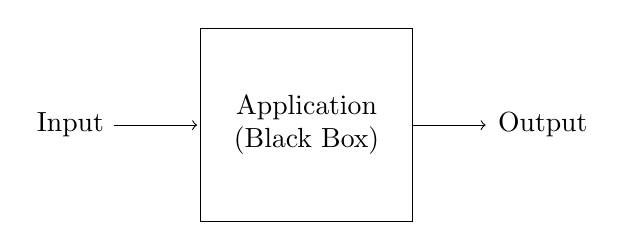
\begin{tikzpicture}[shorten >=1pt, node distance=3cm, auto]
      \node (R0) {Input};
      \node (R1) [right of=R0, minimum height=7em, text width=7em, align=center, draw] {Application\\(Black\ Box)};
      \node (R2) [right of=R1] {Output};
  
      \path[->]
        (R0) edge node {} (R1)
        (R1) edge node {} (R2);
    \end{tikzpicture}
    \caption[Example black-box monitoring]{An example of a black-box monitoring.}\label{fig:example-black-box-monitoring}
\end{figure}

One of the key advantages of black box monitoring is its simplicity and ease of implementation. Since it doesn't require in-depth knowledge of the system internals, it can be quickly deployed across various platforms and systems. This quality fosters wide applicability, accommodating diverse programming languages and system architectures. Furthermore, black box monitoring has a unique focus on the user experience. By simulating user actions and recording the system's responses, it offers a valuable measure of system functionality from a user's perspective. Thus, it is instrumental in ensuring that the system effectively meets the end-users' requirements~\parencite{nidhraBlackBoxWhite2012}. 

However, while the black box approach has its merits, it is not without challenges. One significant limitation is the potential for limited coverage. Since black box monitoring concentrates on the inputs and outputs, it might overlook internal system issues. If a problem doesn't immediately or directly affect the system output, it may remain undetected, only to potentially cause serious issues down the line~\parencite{spillnerSoftwareTestingFoundations2021}. Moreover, black box monitoring could contribute to inefficiency in troubleshooting. A system failure detected by black box testing can be difficult to diagnose and fix due to the lack of visibility into the system internals. Pinpointing the specific area of the system causing the issue may turn into a challenging endeavor.

Despite existing challenges, the prospects for black box monitoring are increasingly optimistic, particularly in our rapidly evolving digital landscape. As customer satisfaction and user experience become paramount in the digital economy, the ability of black box monitoring to accurately reflect system availability and performance from the user's perspective proves invaluable. Moreover, with the advancement of other evolving techniques like eBPF, the scope of black box monitoring continues to expand~\parencite{nevesDetailedBlackboxMonitoring2021}~\parencite{brondolinBlackboxMonitoringApproach2020}. For instance, eBPF's ability to execute custom code in kernel space can provide deeper insights into system operations, thereby enhancing internal observability~\parencite{jonathanBPFUniversalInkernel2014}.

As the IT landscape becomes more complex with microservices and cloud-based applications, understanding the internals of every service can be overwhelming. In such a scenario, black box monitoring's ability to provide a holistic view of system behavior can be highly beneficial. Moreover, in light of growing privacy regulations and data protection measures, black box monitoring's non-invasive approach aligns with the current trends. Focusing on system outputs rather than internals could potentially minimize privacy or data protection concerns.

In conclusion, black box monitoring remains a vital tool for system testing and monitoring, despite its inherent challenges. Its future appears increasingly integrated with AI technologies and aligned with user-centric design principles. Nevertheless, black box monitoring should not be considered a stand-alone solution but rather a component of a comprehensive monitoring strategy that incorporates various techniques to effectively manage system performance.

\section{Prometheus Agent and Blackbox Exporter}

The renowned Prometheus ecosystem provides two important components: the Prometheus Agent and the Blackbox Exporter. These technologies are extensively employed in various enterprises for monitoring applications in testing and production environments. Their widespread adoption is a testament to the reliability and robustness of the Prometheus platform in handling diverse monitoring needs.

The Prometheus Agent is a specialized mode of a standard Prometheus instance aimed at efficient data scraping and remote write as in ~\autoref{fig:prometheus-agent}. Unlike a full-fledged Prometheus server with functionalities like data storage and querying, the Prometheus Agent is streamlined for specific tasks, making it an ideal choice in distributed systems where resource optimization is crucial. This mode is invaluable when a full Prometheus server setup is unnecessary, facilitating a more streamlined and resource-efficient deployment. It is particularly effective in large-scale environments where managing the overhead and complexity of multiple complete Prometheus instances would be impractical~\parencite{prometheusIntroducingPrometheusAgent}.

\begin{figure}[htpb]
    \centering
    % This should probably go into a file in figures/
    \begin{tikzpicture}[
        shorten >=1pt,
        zonetag/.style={align=center, font=\fontsize{10}{10}\color{black!60}\ttfamily},
        node/.style={draw, align=center, minimum height=3em, anchor=west}, 
        zone/.style={draw=black!60}
      ]

      \node (C) at(0, 0) [zonetag] {Cluster};
      \node (PA) [node distance=1cm, below=of C.west, text width=11em, node] {Prometheus\ Agent};
      \node (Apps) [node distance=5cm, right of=PA, text width=5em, node] {Apps};
      \node [zone, fit={(C) (PA) (Apps)}] {};

      \node (G) [node distance=2cm, below=of PA, zonetag] {Global};
      \node (P) [node distance=1cm, below=of G.west, text width=11em, node] {Prometheus/Thanos};
      \node (Am) [node distance=5cm, right of=P, text width=7em, node] {Alertmanager};
      \node [zone, fit={(G) (P) (Am)}] {};
  
      \path[->]
        (P) edge node[below, sloped] {alert} (Am)
        (PA) edge node[auto] {remote write} (P)
        (PA) edge node[below, sloped] {scrape} (Apps);
    \end{tikzpicture}
    \caption[Prometheus Agent]{Prometheus Agent with scrape and remote write.}\label{fig:prometheus-agent}
\end{figure}

The Blackbox Exporter, an essential element of the Prometheus toolkit, is designed to probe external endpoints across multiple protocols, including HTTP/HTTPS, TCP, and ICMP. This capability is fundamental to black box monitoring, enabling the assessment of system health and performance from an external viewpoint without necessitating internal access to the monitored system~\parencite{prometheusBlackboxExporter2023}. The Blackbox Exporter is instrumental in situations where internal monitoring is either not feasible or insufficient, such as in third-party services or in environments where internal metrics are not available or reliable.

Integrating the Prometheus Agent with the Blackbox Exporter fosters a distributed scheduler-executor architecture. This approach allows for a more granular and distributed monitoring framework, which is highly adaptable and can be effectively implemented across various platforms as service (PaaS) clusters with latencies~\parencite{prometheusUnderstandingUsingMultitarget}. Such an architecture bolsters the scalability and resilience of the monitoring system, rendering it suitable for large-scale and intricate environments. This distributed nature enhances the system's ability to scale and ensures a more resilient monitoring setup capable of withstanding node failures and network partitions~\parencite{prometheusIntroducingPrometheusAgent}.

Achieving optimal availability and scalability with the Prometheus Agent and Blackbox Exporter needs additional configuration and management. For the Prometheus Agent, employing relabeling is a crucial horizontal scaling or sharding strategy~\parencite{prometheusHowRelabelingPrometheus}. This method distributes the workload across multiple Prometheus Agent instances with a hidden label with hashed value, augmenting the system's capacity to handle substantial data volumes efficiently. Regarding the Blackbox Exporter, scalability is further enhanced by integrating a load balancer with properly configured scaling parameters, ensuring an even distribution of the probing load and maintaining system performance, even under high demand~\parencite{prometheusIntroducingPrometheusAgent}.

Overall, the active and extensive community surrounding Prometheus plays a significant role in the continuous improvement and reliability of the Prometheus Agent and Blackbox Exporter. This support ensures consistent updates and maintenance, effectively addressing the evolving needs and challenges in the monitoring domain. However, utilizing the Prometheus Agent and Blackbox Exporter to achieve scalability and manageability requires additional configurations and operations. Consequently, automating the scaling and management operations for both the Prometheus Agent and Blackbox Exporter emerges as a critical issue.

\section{Operator Pattern and Prometheus Operator}

The Operator Pattern, defined by the \ac{CNCF}, represents a paradigm shift in Kubernetes, enabling users to automate the maintenance and configuration of applications~\parencite{kubernetesOperatorPattern}. The Prometheus Operator embodies this pattern, serving as an implementation that addresses the practical needs of deploying and managing Prometheus components. Through reconciliation, the Prometheus Operator aligns the deployment's actual state with the user's desired state, streamlining its lifecycle in Kubernetes~\parencite{prometheusoperatorIntroduction2020}.

The Operator Pattern extends Kubernetes' native capabilities by introducing \ac{CRs} and controllers. The operator is the essential software extension that utilize the Kubernetes control plane and API to create, configure, and manage instances of complex stateful applications on behalf of a Kubernetes user~\parencite{dobiesKubernetesOperators}. They encapsulate operational knowledge, automating the management tasks that would typically require manual operations~\parencite{cncfCNCFOperatorWhite}. 

The Prometheus Operator is tailored to simplify the deployment and management of Prometheus within Kubernetes environments. It enables Kubernetes-native deployment and automated management of Prometheus and its associated monitoring components. Key features of the operator include Kubernetes \ac{CRs} for deploying and managing Prometheus, Alertmanager, and so on, streamlined deployment configurations for setting up Prometheus essentials like versions and retention policies, and automatic generation of monitoring target configurations. This approach facilitates easy installation and version upgrades, simplifies configuration management, and ensures seamless integration with existing Kubernetes resources~\parencite{prometheusoperatorIntroduction2020}. 

In terms of current advancements in black box monitoring, the Prometheus Operator supports two \ac{CRs}: Probe and PrometheusAgent. The Probe resource defines monitoring for a set of static targets or ingresses, such as specifying the target for the Blackbox Exporter and the module to be used. On the other hand, PrometheusAgent is responsible for defining a Prometheus agent deployment. This includes configurations like the number of replicas, ScrapeConfigs, and advanced features like sharding~\parencite{prometheusoperatorPrometheusAgentSupport}. Notably, it incorporates the ProbeSelector feature, which links to the previously defined Probe resource, enhancing its functionality and integration~\parencite{prometheusoperatorAPIReference}.

Despite these advancements, a significant gap persists in the management and configuration of the Blackbox Exporter within the Prometheus Operator framework. Specifically, there is no support for using a custom resource definition to manage the Blackbox Exporter. Consequently, users are required to deploy their own instances and modules of the Blackbox Exporter~\parencite{prometheusBlackboxExporter2023}. This limitation underscores the need for more integrated solutions that can simplify the deployment and scaling of the Blackbox Exporter, ensuring it meets the evolving requirements of black box monitoring in complex environments. 

In conclusion, while the Prometheus Operator has made significant strides in enhancing the ease and efficiency of deploying Prometheus in Kubernetes environments, there is still room for improvement, particularly in the realm of black box monitoring. Addressing the current limitations in the management of the Blackbox Exporter will be crucial in realizing the full potential of Prometheus as a comprehensive monitoring solution. 
% !TeX root = ../main.tex
% Add the above to each chapter to make compiling the PDF easier in some editors.

\chapter{Overview}\label{chapter:overview}

\section{Section}

\subsection{Subsection}
% !TeX root = ../main.tex
% Add the above to each chapter to make compiling the PDF easier in some editors.

\chapter{Design}\label{chapter:design}

\section{Prometheus Operator}

Prometheus Operator~\parencite{PrometheusOperator} is an open-source tool designed to simplify the deployment, configuration, and management of Prometheus components in the Kubernetes ecosystem. Prometheus~\parencite{PrometheusMonitoringSystem} has grown in popularity due to its effectiveness in cloud monitoring, making it a cornerstone for developers focusing on reliability and performance. The Prometheus Operator, developed under the support of the \ac{CNCF}, offers cloud deployment and management, aligning seamlessly with the principles and practices of cloud-native computing. 

The primary goal of the Prometheus Operator is to make running Prometheus on the cloud platform as straightforward and efficient as possible. It leverages the container orchestrator's \ac{API}s to offer a scalable and highly available solution that fits the dynamic nature of cloud computing. The operator automates the complex processes of deploying, configuring, and managing Prometheus instances, making it easier for teams that don't have deep expertise in monitoring systems. By introducing \ac{CRD}s representing distinct Prometheus components, such as Alertmanager, PrometheusAgent, and Prometheus itself, the integration lets users define their monitoring requirements with YAML configuration files declaratively. 

Based on the orchestrator's \ac{API}, one of the critical features of the Prometheus Operator is to dynamically discover and manage configurations, such as monitored targets. This dynamic management is crucial in environments where services and workloads constantly change. The operator automates updating Prometheus configurations in response to changes in the cluster, such as adding or removing pods, services, and endpoints. This ensures that monitoring is consistently aligned with the current state of the cluster, providing instant and accurate insights into applications and infrastructure. 

In addition, to enhance the user experience, the Prometheus Operator also supports features like high availability, sharding, etc. To elaborate, for Prometheus and Alertmanager, it is ensured that monitoring and alerting systems remain operational even if individual components fail. For Prometheus Agent, the configuration file is divided into several configurations for multiple agent instances using the hash function, achieving Prometheus Agent sharding for distributing loads. Moreover, the operator also facilitates easy backup and restoration of Prometheus data, integrating with Kubernetes' RBAC model to provide fine-grained access control over monitoring resources. 

In conclusion, the Prometheus Operator enhances cloud monitoring by automating the deployment, configuration, and management of Prometheus. Its dynamic configuration adaptation, high availability, and sharding features increase efficiency and reliability. Therefore, utilizing the Prometheus Operator for robust cloud monitoring solutions in the Amadeus Observability Platform is valuable. 

\section{Prometheus Agent}

\begin{figure}[htpb]
  \centering
  % This should probably go into a file in figures/
  \begin{tikzpicture}[
      shorten >=1pt,
      zonetag/.style={align=center, font=\fontsize{10}{10}\color{black!70}\ttfamily},
      node/.style={draw, align=center, minimum height=3em, anchor=west, rounded corners}, 
      zone/.style={draw=black!60, inner sep=8pt, anchor=west}
    ]

    \node (CRDP) [node distance=7em, text width=7em, node, anchor=base] {CRD\\Probe};
    \node (PO) [node distance=7em, below=of CRDP.base, text width=7em, node, anchor=base] {Prometheus\\Operator};

    \node (conf1) [node distance=4cm, below=of PO.west, text width=7em, node] {Prometheus Config 1};
    \node (conf2) [node distance=8em, right=of conf1.east, text width=7em, node] {Prometheus Config 2};
    \node (PAI1) [node distance=4em, below=of conf1.west, text width=7em, node] {Prometheus Agent Instance};
    \node (PAI2) [node distance=4em, below=of conf2.west, text width=7em, node] {Prometheus Agent Instance};

    \node (PA1Z) [zone, rounded corners, fit={(conf1) (PAI1)}] {};
    \node (PA1) [node distance=6pt, below=of PA1Z, zonetag] {Prometheus Agent 1};
    \node (PA2Z) [zone, rounded corners, fit={(conf2) (PAI2)}] {};
    \node (PA2) [node distance=6pt, below=of PA2Z, zonetag] {Prometheus Agent 2};

    \node (des) [node distance=12em, below=of PA1Z.west, text width=24em, node, dashed, align=left, anchor=west] {The Prometheus Agent achieves sharding on configurations via the "hashmod" relabeling technique. This method involves computing the hash of specified labels, such as URLs. By doing so, the agent could distribute and manage the monitoring load across different instances.};

    \draw[->] (PO) -- node[auto] {Watch} (CRDP);
    \draw[->] (PO) -- node[auto, right, align=center] {Generate configurations with\\additional "hashmod" relabeling} (conf1);
    \draw[->] (PO) -| node[auto, align=center] {} (conf2);
    \draw[<-] (conf1) -- node[auto] {} (PAI1);
    \draw[<-] (conf2) -- node[auto] {} (PAI2);
    \draw[->, dashed] (PA1Z.west) -- +(-1,0) |- (des);
    \draw[->, dashed] (PA2Z.east) -- +(1,0) |- (des);
  \end{tikzpicture}
  \caption[Prometheus Agent Sharding]{Prometheus Agent Sharding Mechanism.}\label{fig:prometheus-agent-sharding}
\end{figure}

The Prometheus Agent~\parencite{PrometheusAgentSupport} represents a simplified, focused approach to monitoring distributed systems, particularly in large-scale and cloud-native environments. As a lightweight variant of the Prometheus instance, the Prometheus Agent is designed to be a highly efficient data collector optimized for forwarding metrics to the Prometheus server or a compatible remote receiver. 

One of the core advantages of the Prometheus Agent lies in its simplicity. Unlike an entire Prometheus server, which includes data storage, querying, and alerting functionalities, the agent is only responsible for scraping metrics and sending them out. This reduction leads to a smaller memory and CPU footprint, critical in resource-constrained environments, making it ideal for edge computing, microservices architectures, and multi-cluster environments. 

In addition, the Prometheus Agent maintains excellent compatibility with the Prometheus ecosystem. This is a crucial consideration for organizations invested in Prometheus-based monitoring. It can scrape metrics in the same Prometheus exposition format, ensuring users integrate the agent seamlessly into the existing monitoring infrastructure. Furthermore, the agent's ability to integrate with service discovery mechanisms in orchestration platforms ensures its dynamically adapting to changes in the monitored environment. 

In conclusion, the Prometheus Agent improves the scalability and reliability of monitoring in large-scale environments, where a central Prometheus server can aggregate and process data from multiple agents. As illustrated in~\autoref{fig:prometheus-agent-sharding}, it achieves this by enabling more efficient horizontal scaling based on scrape configurations, focusing on scraping and forwarding metrics, thus reducing the duplication of storage and computation. Moreover, this highly available architecture boosts the monitoring system's resilience and reliability, as a single agent's failure could have an impact. Overall, the Prometheus Agent is an essential addition to the architecture of the active monitoring platform, offering a scalable and reliable solution for the existing monitoring system. 

\section{Blackbox Exporter and Load Balancing}

Blackbox Exporter~\parencite{BlackboxExporter}, a probing tool for the Prometheus monitoring system, is essential for assessing the performance and availability of services in network environments. It plays an important role in monitoring and diagnosing systems designed for probing endpoints over various protocols like \ac{HTTP}/\ac{HTTPS}, \ac{DNS}, \ac{TCP}, and \ac{ICMP}. 

In complex infrastructures hosting multiple services, it is crucial to integrate the Blackbox Exporter with \ac{OSI} Layer 7 load-balancing solutions such as built-in Load Balancers, OpenShift Routes, Kubernetes Ingress, or \ac{OSI} Layer 3 and 4 solutions like the Service, as depicted in \autoref{fig:openshift-load-balancing}. This integration enables scalable monitoring, ensuring the reliability of the monitoring system as the service count increases. 

\begin{figure}[htpb]
  \centering
  % This should probably go into a file in figures/
  \begin{tikzpicture}[
      shorten >=1pt,
      zonetag/.style={align=center, node distance=1em, font=\fontsize{10}{10}\color{black!70}\ttfamily},
      node/.style={draw, node distance=3em, text width=4em, minimum height=3em, align=center, rounded corners}, 
      zone/.style={draw=black!60, inner sep=8pt}
    ]
    \node (traffic) [node] {Traffic};
    \node (l7) [node, right=of traffic, text width=8em, font=\bfseries] {Load Balancer/\\Ingress/Route};
    \node (l7tag) [zonetag, above=of l7] {OSI Layer 7};
    \node (l34) [node, right=of l7, text width=4em, font=\bfseries] {Service};
    \node (l34tag) [zonetag, above=of l34] {OSI Layer 3/4};
    \node (pod1) [node, above right=of l34] {Pod};
    \node (pod2) [node, right=of l34] {Pod};
    \node (pod3) [node, below right=of l34] {Pod};

    \draw[->] (traffic) -- node[auto] {} (l7);
    \draw[->] (l7) -- node[auto] {} (l34);
    \draw[->] (l34) -- node[auto] {} (pod1);
    \draw[->] (l34) -- node[auto] {} (pod2);
    \draw[->] (l34) -- node[auto] {} (pod3);
  \end{tikzpicture}
  \caption[OpenShift Load Balancing]{Route and Service are responsible for Load Balancing in Openshift.}\label{fig:openshift-load-balancing}
\end{figure}

Furthermore, automatic horizontal scaling significantly enhances resource utilization. Load balancers direct traffic to Blackbox Exporter instances efficiently, adjusted by an orchestrator to prevent resource overuse or depletion. This ensures high availability and fault tolerance, as traffic is rerouted to operational instances in case of failure, ensuring continuous monitoring. Additionally, in dynamic cloud-native environments, this setup facilitates native dynamic service discovery, minimizing manual configuration and simplifying management.

In conclusion, integrating the Blackbox Exporter with load-balancing solutions enhances scalability and reliability in performance monitoring. Load balancing evenly distributes monitoring loads, leading to more accurate performance metrics and easier issue identification. This integration is essential for effectively maintaining network services and is crucial in large-scale deployment and management. 

\section{Argo CD and GitOps}

Argo CD~\parencite{ArgoCDDeclarative}, the declarative GitOps~\parencite{WeaveworksWeavegitopsWeave} continuous delivery tool for Kubernetes, automates the deployment of applications, ensuring they match the desired state configurations stored in Git repositories. GitOps emphasizes infrastructure automation and a pull-based deployment strategy via Git, improving deployment transparency, security, and efficiency. 

Integrating Argo CD and GitOps for managing \ac{CRD}s for PrometheusAgent and Probe on the OpenShift Platform can simplify the deployment and update processes as shown in the \autoref{fig:gitops}. Users commit configuration changes to the Git repository, serving as the single truth source. By monitoring this repository, Argo CD automatically detects changes and communicates with the OpenShift API to update the \ac{CRD}s accordingly, maintaining a continuous synchronization between the desired state in Git and the actual state in the cluster. 

\begin{figure}[htpb]
  \centering
  % This should probably go into a file in figures/
  \begin{tikzpicture}[
      shorten >=1pt,
      zonetag/.style={align=center, font=\fontsize{10}{10}\color{black!70}\ttfamily},
      node/.style={draw, align=center, minimum height=3em, anchor=west, rounded corners}, 
      zone/.style={draw=black!60, inner sep=8pt, anchor=base}
    ]

    \node (user) [node distance=5em, text width=2em, node, circle] {User};
    \node (git) [node distance=5em, text width=2em, node, diamond, right=of user, font=\bfseries] {Git};
    \node (argo) [node distance=7em, text width=6em, node, right=of git, font=\bfseries] {Argo CD};

    \node (api) [node distance=3em, text width=8em, node, below left=of argo] {OpenShift API};

    \node (CRDP) [node distance=3em, text width=12em, node, below=of api] {CRD\\PrometheusAgent/Probe};
    % \node (CRDPA) [node distance=3em, text width=8em, node, ellipse, fill=blue!10, left=of CRDP] {CRD\ PrometheusAgent};
    \node (UZ) [zone, dashed, fit={(CRDP)}] {};
    \node (U) [node distance=6pt, below=of UZ.south, zonetag] {Active Monitoring Platform};

    \node (CZ) [zone, fit={(api) (CRDP) (UZ) (U)}] {};
    \node (C)[node distance=6pt, below=of CZ.south, zonetag] {OpenShift Platform};

    \path[->] (user) edge node[auto, font=\small] {PR merge} (git);
    \path[<-] (git) edge node[auto, font=\small] {Pull Changes} (argo);
    \path[->] (api) edge node[auto, font=\small] {Apply} (CRDP);
    \draw[->] (argo) |- node[auto, font=\small, right]{Webhook Event} (api);
    % \path[->] (api) edge node[auto] {apply} (CRDPA);
  \end{tikzpicture}
  \caption[Utilizing GitOps to manage CRDs]{Utilizing GitOps to manage \ac{CRD}s.}\label{fig:gitops}
\end{figure}

This methodology presents several benefits. Firstly, it enhances security by reducing direct access to the OpenShift environment, as changes are pulled from the repository rather than pushed from external sources. Secondly, it improves deployments' reliability and stability by ensuring they are always aligned with the version-controlled configurations. Additionally, it facilitates an auditable deployment process, enabling easy tracking and rollback of changes. 

However, employing GitOps to manage configurations for Prometheus Agent and Probe has challenges. The learning curve for understanding and setting up GitOps workflows can be steep initially. Moreover, relying on a single source of truth requires strict repository management and version control practices to prevent configuration drift and ensure the repository accurately reflects the deployed environment's state. 

Applying Argo CD and GitOps principles to manage CRDs for PrometheusAgent and Probe within the OpenShift Platform offers a powerful approach to automating deployments. By leveraging Git as the basis of the deployment strategy, users can achieve a more secure, reliable, and transparent infrastructure management process. Despite some challenges, the benefits of adopting a GitOps approach, particularly in complex cloud-native environments, are worthwhile for its value in facilitating efficient and secure deployment workflows. 
% !TeX root = ../main.tex
% Add the above to each chapter to make compiling the PDF easier in some editors.

\chapter{Implementation}\label{chapter:implementation}

\section{Deployment of the Prometheus Operator}

This section aims to detail the preparations and procedures for the setup of the Prometheus Operator. 

\subsection{Modifying CRDs of the Prometheus Operator}

\subsection{Rebuilding the Prometheus Operator}

\subsection{Deploying the Prometheus Operator}

\section{Deployment of the Prometheus Agent}

\subsection{Configuration in CRD}

\subsection{Deploying the CRD: PrometheusAgent}

\section{Deployment of the Blackbox Exporter}

\subsection{Load Balancing from the Openshift Route}

\subsection{Deploying via Helm Chart}

\section{Creating Active Monitoring Configurations}

\subsection{Configuration in CRD}

\subsection{Deploying the CRD: Probe}

\section{GitOps for managing CRDs}

\subsection{Creating Git Repository for CRDs}

\subsection{Registering the Repository in Argo CD}
% !TeX root = ../main.tex
% Add the above to each chapter to make compiling the PDF easier in some editors.

\chapter{Evaluation}\label{chapter:evaluation}

This evaluation study seeks to determine if the design leads to a tolerable overhead compared to the original in-house monitoring application that Amadeus developed. Both applications operate on a private OpenShift Cluster managed by the Amadeus \ac{SRE} team. The primary metrics collected include Openshift Metrics for \ac{CPU}, memory, and network, gathered using cAdvisor or the Network Metrics Daemon~\parencite{redhatAssociatingSecondaryInterfaces}~\parencite{redhatPrometheusClusterMonitoring}. Subsequent sections will outline the evaluation methodology and present the findings from the system analysis.


\section{Methodology}

The evaluation focuses on analyzing system behaviors concerning \ac{CPU} utilization, memory utilization, and network traffic. These three entities are critical for developers to gain insights into system overhead and performance intuitively. Understanding how a system allocates and utilizes its resources, along with how it communicates internally and externally, provides a comprehensive view of its efficiency and scalability.

\subsection{\ac{CPU} Utilization}

For \ac{CPU} utilization analysis within a pod, the metric "container\_cpu\_usage\_seconds\_total" will be utilized. This metric measures the cumulative \ac{CPU} time consumed by a container in seconds. The methodology involves:

\begin{itemize}
    \item Collecting \ac{CPU} usage data over time to understand the baseline and peak \ac{CPU} utilization patterns.
    \item Analyzing the \ac{CPU} consumption in correlation with different applications to identify any potential inefficiencies.
    \item Comparing \ac{CPU} utilization across different applications to assess resource allocation effectiveness.
\end{itemize}

This analysis will help in understanding the \ac{CPU} demands of the applications running in OpenShift Pods and how effectively \ac{CPU} resources are utilized.

\subsection{Memory Utilization}

Memory utilization will be assessed using the "container\_memory\_working\_set\_bytes" metric, which provides the amount of memory actively used by a container, excluding unused pages. The evaluation methodology includes:

\begin{itemize}
    \item Monitoring the working set memory to identify memory usage under different operational conditions.
    \item Investigating memory patterns to ensure that applications operate appropriately and efficiently use memory resources.
    \item Evaluating memory usage trends over time to evaluate resource requirements. 
\end{itemize}

This evaluation aims to highlight memory utilization efficiency and potential areas for optimization within the OpenShift environment.

\subsection{Network I/O}

Network I/O will be analyzed through "container\_network\_receive\_bytes\_total" and "container\_network\_transmit\_bytes\_total" metrics, representing the total bytes received and transmitted by the container network interface, respectively. The methodology involves:

\begin{itemize}
    \item Monitoring inbound and outbound network traffic to identify communication patterns.
    \item Assessing network traffic volume in relation to application activity.
    \item Analyzing network traffic trends to assess data flow efficiency.
\end{itemize}

By examining network I/O, we aim to understand the network performance and efficiency of applications running in OpenShift Pods, highlighting areas for network optimization.

\section{System Analysis}

Prometheus' and Amadeus's solutions feature a similar architecture: the scheduler triggers the prober to carry out monitoring tasks while the prober probes targets. The forthcoming analysis will span 12 hours, focusing on the average hourly values of each metric. Given that the average target count in production environments is nearing 100, the following analysis will address both the scheduler and the prober within the scenario of probing 100 targets. 

\subsection{Scheduler Analysis}

\begin{figure}[htpb]
    \centering
    \pgfplotstableset{col sep=&, row sep=\\}
    % This should probably go into a file in data/
    \pgfplotstableread{
      a & b    \\
      1 & 4.27 \\
      2 & 4.19 \\
      3 & 4.16 \\
      4 & 4.18 \\
      5 & 4.23 \\
      6 & 4.23 \\
      7 & 4.27 \\
      8 & 4.23 \\
      9 & 4.19 \\
      10 & 4.23 \\
      11 & 4.21 \\
      12 & 4.25 \\
    }\cpuA
    \pgfplotstableread{
      a & b    \\
      1 & 2.32 \\
      2 & 2.31 \\
      3 & 2.30 \\
      4 & 2.49 \\
      5 & 2.49 \\
      6 & 2.56 \\
      7 & 2.71 \\
      8 & 2.62 \\
      9 & 2.64 \\
      10 & 2.60 \\
      11 & 2.58 \\
      12 & 2.62 \\
    }\cpuB
    \pgfplotstableread{
      a & b    \\
      1 & 123 \\
      2 & 124 \\
      3 & 123 \\
      4 & 123 \\
      5 & 123 \\
      6 & 124 \\
      7 & 124 \\
      8 & 124 \\
      9 & 125 \\
      10 & 124 \\
      11 & 125 \\
      12 & 125 \\
    }\memA
    \pgfplotstableread{
      a & b    \\
      1 & 267 \\
      2 & 267 \\
      3 & 267 \\
      4 & 267 \\
      5 & 267 \\
      6 & 267 \\
      7 & 267 \\
      8 & 267 \\
      9 & 267 \\
      10 & 267 \\
      11 & 267 \\
      12 & 267 \\
    }\memB
    \pgfplotstableread{
      a & b    \\
      1 & 3.26 \\
      2 & 3.26 \\
      3 & 3.25 \\
      4 & 3.25 \\
      5 & 3.26 \\
      6 & 3.25 \\
      7 & 3.25 \\
      8 & 3.26 \\
      9 & 3.26 \\
      10 & 3.25 \\
      11 & 3.27 \\
      12 & 3.26 \\
    }\netinA
    \pgfplotstableread{
      a & b    \\
      1 & 2.04 \\
      2 & 2.03 \\
      3 & 2.03 \\
      4 & 2.04 \\
      5 & 2.06 \\
      6 & 2.05 \\
      7 & 2.04 \\
      8 & 2.04 \\
      9 & 2.04 \\
      10 & 2.05 \\
      11 & 2.06 \\
      12 & 2.04 \\
    }\netinB
    \pgfplotstableread{
      a & b    \\
      1 & 3.28 \\
      2 & 3.28 \\
      3 & 3.27 \\
      4 & 3.27 \\
      5 & 3.28 \\
      6 & 3.27 \\
      7 & 3.27 \\
      8 & 3.28 \\
      9 & 3.27 \\
      10 & 3.27 \\
      11 & 3.29 \\
      12 & 3.27 \\
    }\netoutA
    \pgfplotstableread{
      a & b    \\
      1 & 9.51 \\
      2 & 9.50 \\
      3 & 9.39 \\
      4 & 9.55 \\
      5 & 9.55 \\
      6 & 9.53 \\
      7 & 9.49 \\
      8 & 9.54 \\
      9 & 9.54 \\
      10 & 9.57 \\
      11 & 9.58 \\
      12 & 9.52 \\
    }\netoutB
    % This should probably go into a file in figures/
    \scalebox{.85}{\begin{tabular}{ c c }
        \begin{tikzpicture}
            \begin{axis}[
              ymin=0,
              grid,
              thick,
              ylabel=CPU (millicore),
              xlabel=Time (hour),
              legend columns=-1,
              legend style={legend pos=south east},
              legend cell align={left}, 
              legend to name=scheduler-analysis
              ]
              \addplot[mark=*, blue] table[x=a, y=b]{\cpuA};
              \addplot[mark=x, red] table[x=a, y=b]{\cpuB};
              \addlegendentry{Prometheus Agent\ \ \ \ };
              \addlegendentry{Amadeus' Scheduler};
            \end{axis}
        \end{tikzpicture} &
        \begin{tikzpicture}
            \begin{axis}[
                ymin=0,
                grid,
                thick,
                ylabel=Memory (MB),
                xlabel=Time (hour)
              ]
              \addplot[mark=*, blue] table[x=a, y=b]{\memA};
              \addplot[mark=x, red] table[x=a, y=b]{\memB};
            \end{axis}
        \end{tikzpicture} \\ 
        \begin{tikzpicture}
            \begin{axis}[
                ymin=0,
                grid,
                thick,
                ylabel=Network In (kB/s),
                xlabel=Time (hour)
              ]
              \addplot[mark=*, blue] table[x=a, y=b]{\netinA};
              \addplot[mark=x, red] table[x=a, y=b]{\netinB};
            \end{axis}
          \end{tikzpicture} &
          \begin{tikzpicture}
            \begin{axis}[
                ymin=0,
                grid,
                thick,
                ylabel=Network Out (kB/s),
                xlabel=Time (hour)
              ]
              \addplot[mark=*, blue] table[x=a, y=b]{\netoutA};
              \addplot[mark=x, red] table[x=a, y=b]{\netoutB};
            \end{axis}
          \end{tikzpicture}  
    \end{tabular}}
    \scalebox{.85}{\ref{scheduler-analysis}}
    \caption[Scheduler Analysis]{Scheduler analysis.}\label{fig:scheduler-analysis}
\end{figure}

The Prometheus Agent and Amadeus' Scheduler perform similar roles but differ in their implementations, with the Prometheus Agent providing additional features. As depicted in the \autoref{fig:scheduler-analysis}, the CPU utilization between the two schedulers shows slight differences due to the minor units in the measurement. Surprisingly, memory utilization by the Prometheus Agent was significantly reduced by approximately 140 MB. Regarding network I/O, given that the measurements are in kB, the differences are relatively inconsequential. Adopting the Prometheus Agent results in an acceptable overhead while substantially decreasing memory consumption. 

\subsection{Prober Analysis}

\begin{figure}[htpb]
  \centering
  \pgfplotstableset{col sep=&, row sep=\\}
  % This should probably go into a file in data/
  \pgfplotstableread{
    a & b    \\
    1 & 16.6 \\
    2 & 16.7 \\
    3 & 16.8 \\
    4 & 16.9 \\
    5 & 16.8 \\
    6 & 16.9 \\
    7 & 16.7 \\
    8 & 16.8 \\
    9 & 17.1 \\
    10 & 16.9 \\
    11 & 17.0 \\
    12 & 16.9 \\
  }\cpuA
  \pgfplotstableread{
    a & b    \\
    1 & 5.82 \\
    2 & 5.92 \\
    3 & 5.87 \\
    4 & 5.91 \\
    5 & 5.91 \\
    6 & 5.89 \\
    7 & 5.91 \\
    8 & 5.95 \\
    9 & 5.99 \\
    10 & 5.84 \\
    11 & 5.97 \\
    12 & 5.94 \\
  }\cpuB
  \pgfplotstableread{
    a & b    \\
    1 & 43.6 \\
    2 & 43.4 \\
    3 & 43.4 \\
    4 & 43.3 \\
    5 & 43.5 \\
    6 & 43.5 \\
    7 & 43.5 \\
    8 & 43.5 \\
    9 & 44.0 \\
    10 & 43.8 \\
    11 & 44.0 \\
    12 & 44.1 \\
  }\memA
  \pgfplotstableread{
    a & b    \\
    1 & 297 \\
    2 & 297 \\
    3 & 297 \\
    4 & 297 \\
    5 & 297 \\
    6 & 297 \\
    7 & 297 \\
    8 & 297 \\
    9 & 297 \\
    10 & 297 \\
    11 & 297 \\
    12 & 297 \\
  }\memB
  \pgfplotstableread{
    a & b    \\
    1 & 30.1 \\
    2 & 30.1 \\
    3 & 30.1 \\
    4 & 30.1 \\
    5 & 30.0 \\
    6 & 30.1 \\
    7 & 30.1 \\
    8 & 30.2 \\
    9 & 30.2 \\
    10 & 30.1 \\
    11 & 30.1 \\
    12 & 30.2 \\
  }\netinA
  \pgfplotstableread{
    a & b    \\
    1 & 13.5 \\
    2 & 13.5 \\
    3 & 13.5 \\
    4 & 13.5 \\
    5 & 13.5 \\
    6 & 13.5 \\
    7 & 13.3 \\
    8 & 13.3 \\
    9 & 13.5 \\
    10 & 13.5 \\
    11 & 13.5 \\
    12 & 13.5 \\
  }\netinB
  \pgfplotstableread{
    a & b    \\
    1 & 11.2 \\
    2 & 11.2 \\
    3 & 11.3 \\
    4 & 11.3 \\
    5 & 11.2 \\
    6 & 11.3 \\
    7 & 11.3 \\
    8 & 11.3 \\
    9 & 11.3 \\
    10 & 11.3 \\
    11 & 11.3 \\
    12 & 11.3 \\
  }\netoutA
  \pgfplotstableread{
    a & b    \\
    1 & 9.79 \\
    2 & 9.78 \\
    3 & 9.76 \\
    4 & 9.78 \\
    5 & 9.78 \\
    6 & 9.79 \\
    7 & 9.61 \\
    8 & 9.62 \\
    9 & 9.78 \\
    10 & 9.77 \\
    11 & 9.78 \\
    12 & 9.76 \\
  }\netoutB
  % This should probably go into a file in figures/
  \scalebox{.85}{\begin{tabular}{ c c }
      \begin{tikzpicture}
          \begin{axis}[
              ymin=0,
              grid,
              thick,
              ylabel=CPU (millicore),
              xlabel=Time (hour),
              legend columns=-1,
              legend style={legend pos=south east},
              legend cell align={left}, 
              legend to name=prober-analysis,
            ]
            \addplot[mark=*, blue] table[x=a, y=b]{\cpuA};
            \addplot[mark=x, red] table[x=a, y=b]{\cpuB};
            \addlegendentry{Blackbox Exporter\ \ \ \ };
            \addlegendentry{Amadeus' HTTP Prober};
          \end{axis}
      \end{tikzpicture} &
      \begin{tikzpicture}
          \begin{axis}[
              ymin=0,
              grid,
              thick,
              ylabel=Memory (MB),
              xlabel=Time (hour),
            ]
            \addplot[mark=*, blue] table[x=a, y=b]{\memA};
            \addplot[mark=x, red] table[x=a, y=b]{\memB};
          \end{axis}
      \end{tikzpicture} \\ 
      \begin{tikzpicture}
          \begin{axis}[
              ymin=0,
              legend style={legend pos=south east},
              grid,
              thick,
              ylabel=Network In (kB/s),
              xlabel=Time (hour),
              legend cell align={left}
            ]
            \addplot[mark=*, blue] table[x=a, y=b]{\netinA};
            \addplot[mark=x, red] table[x=a, y=b]{\netinB};
          \end{axis}
        \end{tikzpicture} &
      \begin{tikzpicture}
        \begin{axis}[
            ymin=0,
            grid,
            thick,
            ylabel=Network Out (kB/s),
            xlabel=Time (hour),
          ]
          \addplot[mark=*, blue] table[x=a, y=b]{\netoutA};
          \addplot[mark=x, red] table[x=a, y=b]{\netoutB};
        \end{axis}
      \end{tikzpicture}
  \end{tabular}}
  \scalebox{.85}{\ref{prober-analysis}}
  \caption[Prober Analysis]{Prober analysis.}\label{fig:prober-analysis}
\end{figure}

The Blackbox Exporter, capable of conducting customized probes across different protocols, contrasts with Amadeus' HTTP Prober's limitation to only HTTP probes. For a fair comparison, only the HTTP module is used in the Blackbox Exporter. \autoref{fig:prober-analysis} shows the Blackbox Exporter's CPU usage is slightly higher than Amadeus' by about 10 millicores, a minor increase justified by its extended features and considered acceptable. Notably, it also offers a substantial memory usage improvement of approximately 250 MB. Although its network input is double that of its counterpart, investigations reveal this is due to the Prometheus Agent's more detailed HTTP GET requests, which are not expected to cause issues, even when scaling up to 10 or 100 times the number of targets due to the lightweight nature of these requests. In summary, the minor increases in CPU and network input by the Blackbox Exporter are more than compensated for by considerable memory savings, making it a fully acceptable solution. 

\section{Overhead Analysis}

This overhead analysis evaluates the escalating load rate as the target number increases from 100 to 1000. Utilizing these findings could enhance the use of \ac{HPA} by identifying appropriate threshold metrics. All metrics were recorded as hourly averages for each target number, expected to increase proportionally with the target number in theory: 

\begin{figure}[htpb]
  \centering
  \pgfplotstableset{col sep=&, row sep=\\}
  % This should probably go into a file in data/
  \pgfplotstableread{
    a & b    \\
    100 & 4.13 \\
    200 & 5.46 \\
    300 & 6.95 \\
    400 & 10.0 \\
    500 & 11.7 \\
    600 & 13.2 \\
    700 & 14.3 \\
    800 & 16.1 \\
    900 & 20.2 \\
    1000 & 22.0 \\
  }\cpuA
  \pgfplotstableread{
    a & b    \\
    100 & 16.8 \\
    200 & 32.7 \\
    300 & 48.6 \\
    400 & 63.8 \\
    500 & 79.7 \\
    600 & 95.9 \\
    700 & 112 \\
    800 & 128 \\
    900 & 144 \\
    1000 & 160 \\
  }\cpuB
  \pgfplotstableread{
    a & b    \\
    100 & 245 \\
    200 & 328 \\
    300 & 426 \\
    400 & 496 \\
    500 & 610 \\
    600 & 720 \\
    700 & 766 \\
    800 & 836 \\
    900 & 919 \\
    1000 & 1075 \\
  }\memA
  \pgfplotstableread{
    a & b    \\
    100 & 92.7 \\
    200 & 101 \\
    300 & 110 \\
    400 & 124 \\
    500 & 133 \\
    600 & 145 \\
    700 & 155 \\
    800 & 191 \\
    900 & 200 \\
    1000 & 209 \\
  }\memB
  \pgfplotstableread{
    a & b    \\
    100 & 3.25 \\
    200 & 6.31 \\
    300 & 9.36 \\
    400 & 12.5 \\
    500 & 15.5 \\
    600 & 18.6 \\
    700 & 21.7 \\
    800 & 24.7 \\
    900 & 27.7 \\
    1000 & 30.8 \\
  }\netinA
  \pgfplotstableread{
    a & b    \\
    100 & 30.3 \\
    200 & 60.5 \\
    300 & 90.6 \\
    400 & 121 \\
    500 & 150 \\
    600 & 182 \\
    700 & 211 \\
    800 & 241 \\
    900 & 272 \\
    1000 & 302 \\
  }\netinB
  \pgfplotstableread{
    a & b    \\
    100 & 3.29 \\
    200 & 6.34 \\
    300 & 9.35 \\
    400 & 12.4 \\
    500 & 15.4 \\
    600 & 18.5 \\
    700 & 21.5 \\
    800 & 24.5 \\
    900 & 27.5 \\
    1000 & 30.5 \\
  }\netoutA
  \pgfplotstableread{
    a & b    \\
    100 & 11.6 \\
    200 & 19.1 \\
    300 & 26.6 \\
    400 & 33.8 \\
    500 & 41.4 \\
    600 & 49.2 \\
    700 & 56.6 \\
    800 & 64.2 \\
    900 & 71.8 \\
    1000 & 79.4 \\
  }\netoutB
  % This should probably go into a file in figures/
  \scalebox{.85}{\begin{tabular}{ c c }
      \begin{tikzpicture}
          \begin{axis}[
            ymin=0,
            grid,
            thick,
            ylabel=CPU (millicore),
            xlabel=Target Number,
            legend columns=-1,
            legend style={legend pos=south east},
            legend cell align={left}, 
            legend to name=overhead-analysis
            ]
            \addplot[mark=*, blue] table[x=a, y=b]{\cpuA};
            \addplot[mark=x, red] table[x=a, y=b]{\cpuB};
            \addlegendentry{Prometheus Agent\ \ \ \ };
            \addlegendentry{Blackbox Exporter};
          \end{axis}
      \end{tikzpicture} &
      \begin{tikzpicture}
          \begin{axis}[
              ymin=0,
              grid,
              thick,
              ylabel=Memory (MB),
              xlabel=Target Number
            ]
            \addplot[mark=*, blue] table[x=a, y=b]{\memA};
            \addplot[mark=x, red] table[x=a, y=b]{\memB};
          \end{axis}
      \end{tikzpicture} \\ 
      \begin{tikzpicture}
          \begin{axis}[
              ymin=0,
              grid,
              thick,
              ylabel=Network In (kB/s),
              xlabel=Target Number
            ]
            \addplot[mark=*, blue] table[x=a, y=b]{\netinA};
            \addplot[mark=x, red] table[x=a, y=b]{\netinB};
          \end{axis}
        \end{tikzpicture} &
        \begin{tikzpicture}
          \begin{axis}[
              ymin=0,
              grid,
              thick,
              ylabel=Network Out (kB/s),
              xlabel=Target Number
            ]
            \addplot[mark=*, blue] table[x=a, y=b]{\netoutA};
            \addplot[mark=x, red] table[x=a, y=b]{\netoutB};
          \end{axis}
        \end{tikzpicture}  
  \end{tabular}}
  \scalebox{.85}{\ref{overhead-analysis}}
  \caption[Overhead Analysis]{Overhead analysis.}\label{fig:overhead-analysis}
\end{figure}

As shown in the above \autoref{fig:overhead-analysis}, all metrics demonstrate a consistent linear growth trend with each addition of 100 targets. Initially, the Prometheus Agent exhibits significant memory usage and a higher rate of increase, attributed to its role in scheduling probes, which involves managing numerous scraping jobs and their associated configurations. Therefore, utilizing the memory metrics from the Prometheus Agent for \ac{HPA} is a reasonable choice. Conversely, the behavior of the Blackbox Exporter differs from the Prometheus Agent. It displays a modest upward trend in memory usage alongside more pronounced CPU and network utilization increases. Notably, the growth rates for CPU and network usage are comparable, indicating that the overhead is primarily relevant to network-related tasks. Thus, CPU metrics are suitable as threshold indicators for the Blackbox Exporter. 

\section{Scraping Analysis}

This analysis assesses the efficiency of the Prometheus Agent's scraping approach by tracking the "Network In" metric of the Prober, which can be regarded as an indicator of the traffic generated by the Scheduler's probing requests. The traffic is quantified as the average per minute, with the following figure metrics over 30 minutes: 

\begin{figure}[htpb]
  \centering
  \pgfplotstableset{col sep=&, row sep=\\}
  % This should probably go into a file in data/
  \pgfplotstableread{
    a & b    \\
    1 & 33.7 \\
    2 & 39.8 \\
    3 & 30.8 \\
    4 & 27.1 \\
    5 & 28.4 \\
    6 & 32.1 \\
    7 & 32.1 \\
    8 & 32.3 \\
    9 & 25.4 \\
    10 & 19.3 \\
    11 & 30.4 \\
    12 & 41.7 \\
    13 & 31.6 \\
    14 & 22.4 \\
    15 & 40.4 \\
    16 & 18.1 \\
    17 & 30.7 \\
    18 & 39.5 \\
    19 & 30.6 \\
    20 & 22.7 \\
    21 & 31.2 \\
    22 & 36.4 \\
    23 & 25.7 \\
    24 & 23.1 \\
    25 & 33.6 \\
    26 & 29.3 \\
    27 & 31.1 \\
    28 & 40.4 \\
    29 & 14.6 \\
    30 & 43.0 \\
  }\netinA
  \pgfplotstableread{
    a & b    \\
    1 & 32.1 \\
    2 & 0 \\
    3 & 26.8 \\
    4 & 0 \\
    5 & 26.8 \\
    6 & 0 \\
    7 & 26.7 \\
    8 & 0 \\
    9 & 26.7 \\
    10 & 0 \\
    11 & 26.7 \\
    12 & 0 \\
    13 & 26.8 \\
    14 & 0 \\
    15 & 26.8 \\
    16 & 0 \\
    17 & 26.8 \\
    18 & 0 \\
    19 & 26.8 \\
    20 & 0 \\
    21 & 26.8 \\
    22 & 0 \\
    23 & 26.8 \\
    24 & 0 \\
    25 & 26.7 \\
    26 & 0 \\
    27 & 26.7 \\
    28 & 0 \\
    29 & 26.8 \\
    30 & 0 \\
  }\netinB
  % This should probably go into a file in figures/
  \scalebox{.85}{\begin{tikzpicture}
    \begin{axis}[
        ymin=0,
        legend style={legend pos=south east},
        grid,
        thick,
        ylabel=Net In (kB/s),
        xlabel=Time (min)
      ]
      \addplot[mark=*, blue] table[x=a, y=b]{\netinA};
      \addplot[mark=x, red] table[x=a, y=b]{\netinB};
      \addlegendentry{Net In - Blackbox Exporter};
      \addlegendentry{Net In - Amadeus' Prober};
    \end{axis}
  \end{tikzpicture}}
  \caption[Scrape Analysis]{Scrape Analysis.}\label{fig:scrape-analysis}
\end{figure}

As demonstrated in the \autoref{fig:scrape-analysis}, it is evident that there is no zero traffic in the Blackbox Exporter within 30 minutes, in contrast to Amadeus' Prober, which exhibits regular saw-tooth traffic patterns touching the bottom, indicating periodical drops in traffic to zero. This observation suggests that Prometheus Agent spreads scatters across the time interval, resulting in more optimized and spread network traffic. 
% !TeX root = ../main.tex
% Add the above to each chapter to make compiling the PDF easier in some editors.

\chapter{Related Work}\label{chapter:related_work}

Modern IT infrastructure management, monitoring, and analytics platforms ensure system reliability and performance. Some industries, like Amadeus, design and customize their solution, while some employ mature commercial, robust solutions from renowned enterprises such as Datadog. The upcoming section will introduce two representative solutions relative to active monitoring: the solution developed and used internally by Amadeus since 2021 and another solution driven by Datadog's synthetic monitoring~\parencite{datadogSyntheticMonitoring}. 

\section{Amadeus' Active Monitoring}

\begin{figure}[htpb]
  \centering
  % This should probably go into a file in figures/
  \begin{tikzpicture}[
      shorten >=1pt,
      zonetag/.style={align=center, font=\fontsize{10}{10}\color{black!60}\ttfamily, anchor=west},
      node/.style={draw, align=center, minimum height=3em, anchor=west, rounded corners}, 
      zone/.style={draw=black!60, inner sep=8pt, anchor=base}
    ]

    \node (user) [node distance=5em, text width=3em, node, circle] {User};

    \node (operator) [node distance=3em, text width=8em, node, below=of user] {Operator\\(Handle CR)};
    \node (scheduler) [node distance=3em, text width=8em, node, below=of operator] {Scheduler\\(Manage Probers)};
    \node (prober1) [node distance=3em, text width=8em, node, below=of scheduler] {HTTP Prober};
    \node (prober2) [node distance=3em, text width=8em, node, left=of prober1] {TCP Prober};
    \node (prober3) [node distance=3em, text width=8em, node, right=of prober1] {HTTPS Prober};
    \node (target1) [node distance=3em, text width=8em, node, below=of prober1] {Target B};
    \node (target2) [node distance=3em, text width=8em, node, left=of target1] {Target A};
    \node (target3) [node distance=3em, text width=8em, node, right=of target1] {Target C};

    \node (CZ) [zone, fit={(operator) (scheduler) (prober1) (prober2) (prober3) (target1) (target2) (target3)}] {};
    \node (C)[node distance=6pt, above=of CZ.north west, zonetag] {OpenShift Cluster};

    \path[->] (user) edge node[auto, midway] {Create CR} (operator);
    \path[->] (operator) edge node[auto] {Configure} (scheduler);
    \path[->] (scheduler) edge node[auto] {Trigger} (prober1);
    \path[->] (scheduler) edge node[auto] {Trigger} (prober2);
    \path[->] (scheduler) edge node[auto] {Trigger} (prober3);
    \path[->] (prober1) edge node[auto] {} (target1);
    \path[->] (prober2) edge node[auto] {Probe} (target1);
    \path[->] (prober3) edge node[auto] {Probe} (target3);
    \path[->] (prober3) edge node[auto] {Probe} (target2);
  \end{tikzpicture}
  \caption[Amadeus' Active Monitoring]{Amadeus' Active Monitoring.}\label{fig:amadeus-active-monitoring}
\end{figure}

Inspired by the Blackbox Monitoring principles, Amadeus developed the active monitoring system by integrating the Operator pattern, aiming for a simple cloud monitoring solution. As shown in \autoref{fig:amadeus-active-monitoring}, this system is architecturally composed of three pivotal elements: the operator, the scheduler, and the prober. This design facilitates a lightweight yet practical approach to cloud-native monitoring. 

Users initially tailor their monitoring setup using \ac{CR}. The operator is key in interpreting these \ac{CR}s to establish and maintain the scheduler's monitoring configuration. This approach highlights the system's flexibility, allowing users to define monitoring configurations that meet their specific needs. 

The scheduler is central to the system's functionality, orchestrating the monitoring process. It is responsible for initiating monitoring requests, per the configurations detailed in the \ac{CR}s, and coordinating with the probers to gather the requisite data. The probers, designed as workers, are tasked with executing the monitoring by probing the targeted services and directing the collected data back to the scheduler. This component-driven approach ensures a comprehensive monitoring cycle. 

Despite its sound design, the system's limitations restrain its potency, particularly in large-scale applications. Notably, the architecture presents a single point of failure at the scheduler, posing risks of data collection interruptions and potential traffic bottlenecks. The lack of scalability poses these challenges, making it difficult to efficiently monitor a vast array of distributed services across multiple clusters. 

\section{Datadog's Synthetic Monitoring}

\begin{figure}[htpb]
  \centering
  % This should probably go into a file in figures/
  \begin{tikzpicture}[
      shorten >=1pt,
      zonetag/.style={align=center},
      node/.style={draw, align=center, minimum height=3em, anchor=west, rounded corners}, 
      zone/.style={draw=black!60, inner sep=8pt, anchor=base}
    ]

    \node (datadog) [node distance=5em, text width=6em, node] {Datadog};

    \node (agent1) [node distance=4em, text width=4em, node, below left=of datadog] {Agent};
    \node (target1) [node distance=3em, text width=4em, node, left=of agent1] {Target};
    \node (target2) [node distance=2em, text width=4em, node, below=of target1] {Target};
    \node (target3) [node distance=2em, text width=4em, node, below=of target2] {Target};
    \node (CZ1) [zone, fit={(agent1) (target1) (target2) (target3)}] {};
    \draw[->] (datadog) -| node[auto, left] {Pull Metrics} (agent1);
    \draw[->] (agent1) edge node[auto, below] {} (target1);
    \draw[->] (agent1) |- node[auto, right] {API Test} (target2);
    \draw[->] (agent1) |- node[auto] {} (target3);

    \node (agent2) [node distance=4em, text width=4em, node, below right=of datadog] {Agent};
    \node (target4) [node distance=3em, text width=4em, node, right=of agent2] {Target};
    \node (target5) [node distance=2em, text width=4em, node, below=of target4] {Target};
    \node (target6) [node distance=2em, text width=4em, node, below=of target5] {Target};
    \node (CZ2) [zone, fit={(agent2) (target4) (target5) (target6)}] {};
    \draw[->] (datadog) -| node[auto, right]{Pull Metrics} (agent2);
    \draw[->] (agent2) edge node[auto, below] {} (target4);
    \draw[->] (agent2) |- node[auto, left] {API Test} (target5);
    \draw[->] (agent2) |- node[auto] {} (target6);

    \draw[-] (agent1) edge node[auto] { Internal Network} (agent2);

  \end{tikzpicture}
  \caption[Datadog's Synthetic Monitoring]{Datadog's Synthetic Monitoring.}\label{fig:datadog-synthetic-monitoring}
\end{figure}

% In the realm of modern IT infrastructure management, monitoring and analytics platforms play an integral role in ensuring system reliability and performance. Among the existing solutions, Datadog has emerged as a prominent player, known for its robust functionalities and capabilities~\parencite{datadogSyntheticMonitoring}. In the context of this project, which aims to design a dedicated and distributed active monitoring system, understanding Datadog's approach and technology is pivotal. 

As an integrated platform for monitoring, Datadog collects and analyzes data from multiple sources, offering a unified view of an organization's IT infrastructure. A standout feature of Datadog is the Synthetic Monitoring (see \autoref{fig:datadog-synthetic-monitoring}), which is particularly applicable for active monitoring~\parencite{datadogSyntheticMonitoring} [Data]. This feature simulates requests and actions, thereby offering insights into the performance of APIs across various network layers, from backend to frontend~\parencite{datadogAPITests}~\parencite{datadogBrowserTests}. 

There are two distinct elements of Datadog's Synthetic Monitoring that are of particular interest: API Tests and Browser Tests~\parencite{datadogAPITests}~\parencite{datadogBrowserTests}. API Tests actively probe target services, gathering their statuses and metrics. These tests offer a snapshot of the availability of the monitored services, a crucial factor in any active monitoring system. In Datadog's implementation, API Tests form the bulk of the monitoring process, thereby highlighting their importance. Browser Tests, on the other hand, execute defined scenarios on target services using a chosen browser. This essentially reproduces the actions of a user, providing experiential feedback about the services. This user-centric approach complements the more technical data gathered by the API Tests, contributing to a more holistic view of the system's health. 

When it comes to monitoring availability, it is crucial to decide the position of source endpoints that proceed with monitoring~\parencite{datadogRunSyntheticTests}. Datadog provides the feature to customize private locations to execute Synthetic Monitoring. By installing Docker containers as private endpoints in desired locations, Synthetic Monitoring, including API Tests and Browser Tests, can employ these remote endpoints as its starting point. 

While Datadog's synthetic monitoring approach presents a well-rounded solution, it operates primarily within a centralized model in terms of the agents' side. To elaborate, monitoring targets from a private location requires an installed agent in the same cluster, and the agent could be a single point of failure. 
% !TeX root = ../main.tex
% Add the above to each chapter to make compiling the PDF easier in some editors.

\chapter{Summary and Conclusion}\label{chapter:summary_and_conclusion}

\section{Section}

\subsection{Subsection}
% !TeX root = ../main.tex
% Add the above to each chapter to make compiling the PDF easier in some editors.

\chapter{Future Work}\label{chapter:future_work}

No matter how IT industries evolve, advancing system monitoring techniques cannot be overlooked. The thesis has laid the groundwork for understanding and enhancing the observability of complex IT infrastructures with Active Monitoring, emphasizing utilizing the Prometheus Operator and Blackbox Exporter. Nonetheless, a vast expanse of uncharted territory remains ripe for exploration. The following paragraphs introduce promising directions for future research, each offering the potential to significantly refine and advance our current monitoring capabilities. These directions include the automation of Blackbox Exporter configurations, developing interfaces for custom probers, and integrating eBPF programs for low-cost, high-precision monitoring. 

A promising area for further investigation involves enhancing the Prometheus Operator's functionality, particularly in managing the Blackbox Exporter's configuration through \ac{CRD}s. Automating this aspect would mark a significant leap toward more manageable and efficient monitoring systems, reducing the manual overhead for maintainers and aligning the Blackbox Exporter more closely with the automated, operator-managed setup of the Prometheus Agent. This evolution toward automated configurations promises to elevate the efficiency of monitoring operations and ensure a higher degree of flexibility and ease of maintenance. 

Exploring an interface for creating and managing custom probers within the Blackbox Exporter framework represents another direction for research. The limitation to officially supported probers restricts the tool's applicability across diverse monitoring scenarios. By developing a customizable interface, users could employ monitoring solutions to their specific needs, significantly enhancing the tool's versatility and the relevance of the data it collects. This advancement would enable more delicate monitoring approaches, allowing for a broader application spectrum and more targeted data collection strategies. 

Furthermore, the potential integration of eBPF programs into the Blackbox Exporter offers an exciting prospect for the future of monitoring. eBPF, known as Extended Berkeley Packet Filter, is a technology that allows efficient performance monitoring within the kernel space without requiring traditional overheads. Leveraging eBPF's ability to perform low-level, low-cost analyses could transform the observability landscape of Active Monitoring, providing insights into system performance with minimal overhead. This approach could lead to more effective and efficient monitoring strategies, enabling a deeper understanding of system behaviors and facilitating more fine-grained performance improvement. 

Beyond these specific areas, the continuous evolution of cloud computing and container technology presents ongoing opportunities for the refinement of monitoring strategies and tools. The integration of advanced machine learning techniques for predictive monitoring, the development of finer-grained tools for microservices architectures, and the investigation of automated system recovery mechanisms based on monitoring data are critical areas where future research could drive significant improvements. By pushing the boundaries in these directions, the field can anticipate and adapt to the changing landscape of IT infrastructures, ensuring that monitoring solutions remain robust, effective, and aligned with the needs of modern technologies. 

In sum, the future work mentioned here is not just an extension of this thesis but a roadmap for advancing system monitoring into new realms of efficiency, flexibility, and observability. By pursuing these research directions, the field can look forward to monitoring solutions that are not only more capable but also more adapted to the dynamic complexities of modern IT environments. 

\appendix{}

\microtypesetup{protrusion=false}

\addchap{Abbreviations}
\begin{acronym}
	\itemsep-.25\baselineskip
	\acro{ACS}[ACS]{Amadeus Cloud Service}
	\acro{AI}[AI]{Artificial Intelligence}
	\acro{CNCF}[CNCF]{Cloud Native Computing Foundation}
	\acro{CRs}[CRs]{Custom Resources}
	\acro{CRD}[CRD]{Custom Resource Definition}
	\acro{ML}[ML]{Machine Learning}
	\acro{OBE}[OBE]{Open Back End}
	\acro{SI}[SI]{Service Integration}
	\acro{SLA}[SLA]{Service Level Agreement}
	\acro{TUM}[TUM]{Technical University of Munich}
	% TODO: add acronyms
\end{acronym}

\listoffigures{}
\listoftables{}
\microtypesetup{protrusion=true}
\printbibliography{}

\end{document}
